\chapter{Small Sphere Experiment}
\label{chap:SmallSphere}

\textit{The work presented here has been presented as an invited oral presentation by Lindsay MacDonald at AIC 2017 \citep{macdonald_melanopsin_2017}\footnote{The proceedings are not currently available online, though a note at \url{https://aic-color.org/page-18077} suggests that they will soon be available.}.}


\section{Summary}

\hl{insert summary.}

This study was approved by the \gls{UCL} Ethics committee (Project ID Number: 9357/003), application attached as Appendix \ref{app:ethics3}. Code and data are provided: \url{https://github.com/da5nsy/Small-Sphere}.

\section{Introduction}

% why this experiment? Response to issues in large sphere
% - luminance
% - too many variables
% research question

This experiment was performed to develop upon the Large Sphere experiment (Chapter \ref{chap:LargeSphere}) by narrowing down the number of variables and more directly exploring the question of whether melanopsin plays a role in colour constancy. This was achieved using a similar experimental set-up to the previous experiment, with several key alterations:

\begin{enumerate}
    \item Instead of 16 surround conditions, only two were included.
    \begin{enumerate}
        \item These two conditions were generated through use of narrowband LEDs rather than filtered white light, designed to be perceptual metamers for each observer, but with maximally different levels of melanopic activation.
    \end{enumerate}
    \item Instead of 16 lightness conditions, only 5 were included.
    \item The sphere used was smaller, and the inner surface was painted with a higher reflectance paint, with the hope of increasing the level of adapting radiation.
    \item Three observers were tested (the author and two colleagues of a similar age), with repeats of each condition.
\end{enumerate}

Further details on all of the above amendments will be included in the following sections. 

The null hypothesis that this experiment aims to test is that melanopsin activation does not alter an observers perceptual white point.

\section{Materials and Methods}

\subsection{Hardware}

The sphere used in this experiment was 400mm in diameter, with ports of similar functions to those in the Large Sphere. On one side there is a padded port for an observer's face. Mirroring this is a small aperture through which an LCD screen is visible. At the top of the sphere was a port through which adapting illumination was provided. An additional port, on the observer's side of the base, was added such that the illumination provided to the sphere could be unobtrusively monitored throughout experiments.

\begin{figure}[htbp]
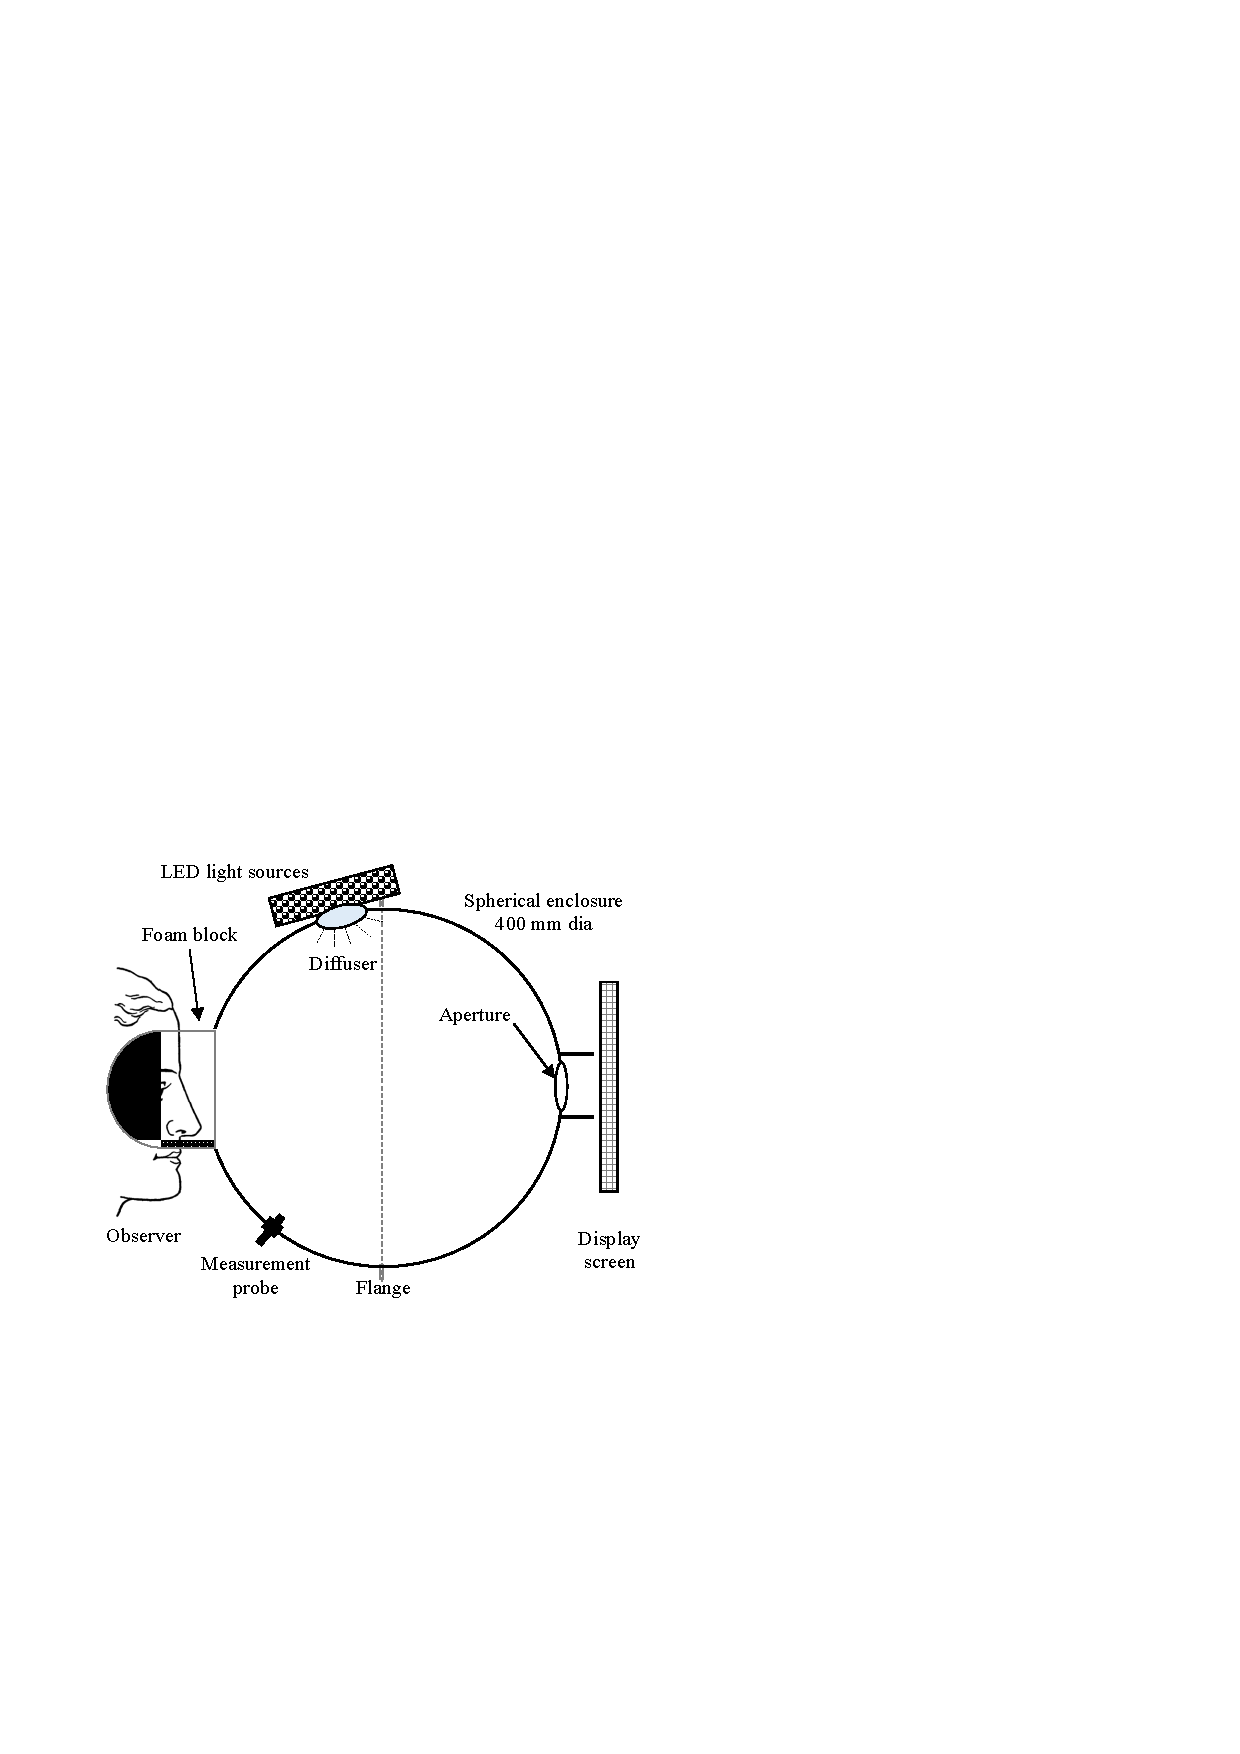
\includegraphics[max width=\textwidth,center]{figs/SmallSphere/diagram.pdf}
\caption{The small sphere set up, reproduced from \citet{macdonald_melanopsin_2017}, courtesy of Lindsay MacDonald.}
\label{fig:diagram}
\end{figure}

\subsection{The sphere}

% how big was the fixation?

% diagram 
% photo

The sphere used in this experiment was smaller than that in the previous experiments (hence the experiment short-hand names) and this served several purposes. The illumination in the Large Sphere had been rather low, partly such that rod interactions would be made visible, and partly due to practical limitations. The grey paint on the interior of the Large Sphere was chosen such to limit specular reflections, but it meant that overall illumination levels were very low. In the small sphere, it was hoped that by reducing the size of the sphere it would be possible to increase the level of illumination, as it would be spread across a smaller surface. Additionally, of practical concern, it was easier to find experimental space for a smaller sphere.

Several paints were trialled for use in the small sphere. The required conditions were that they were available as a spray, and provided as `matt white'. Sample patches were sprayed upon a piece of opaque perspex to assess finish and spectral reflectance. It was seen as beneficial if: the finish had a very fine grain and as little gloss to it as possible, the surface reflectance was high and the \gls{SRF} was as uniform across the spectrum as possible. It was also considered a requisite requirement that any paint should not include any fluorescent whitening agents (such as can be seen in the `white paper' shown in Figure \ref{fig:spray}).

Measurements of the \glspl{SRF} of the 8 tested spray-paints, and further details of the spray-paints themselves, can be seen in Figure \ref{fig:spray}. Measurements were made with a \gls{PR650}, illuminated at 45$^{\circ}$ and measured at 90$^{\circ}$. It can be seen that Montana Gold Sh. White Cream and Pebble, along with MTN 94 RV-198 are either too low in reflectance, or not spectrally uniform enough. The two with the most desirable finishes were the Flame Blue and MTN Water Based paints. The MTN Water Based paint was chosen due to its particularly fine-grain finish.

%The sharp drop off in the \glspl{SRF} suggest that most of the tested paints were titanium-based (based on comparisons to measurements made by \citet{cosentino_fors_2014})\footnote{It is unfortunate in some ways that the \glspl{SRF} drop so rapidly around 400nm, as this means that the one of the chosen LEDs with a peak output of around 400nm will lose a great deal of its power in the interaction with the paint. On the other hand - this decreases the risk to the observer of being exposed to exessive amounts of short wavelength radiation.}.  

\begin{figure}[htbp]
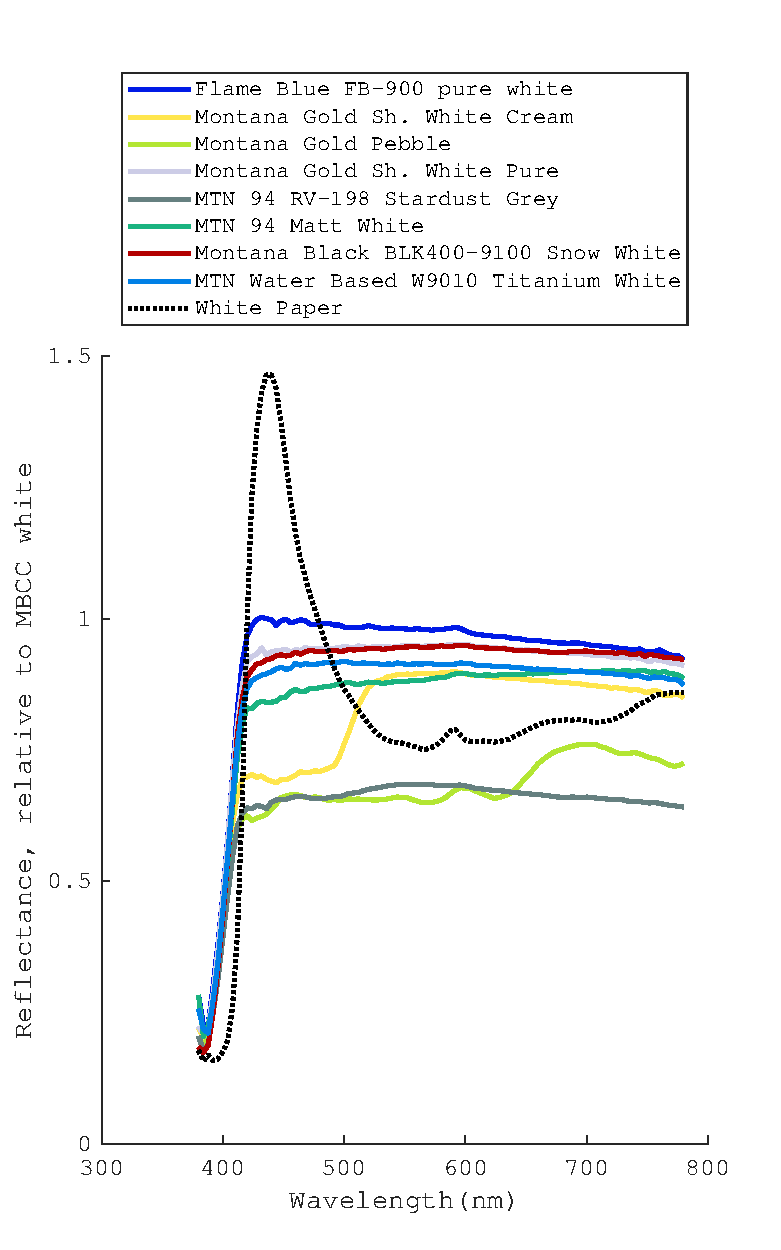
\includegraphics[max width=0.9\textwidth,center]{figs/SmallSphere/VisualiseSPDs_result.pdf}
\caption{The \glspl{SRF} of the 8 tested paints (relative to the white patch of a MacBeth Colour Checker card) with an additional measurement of a piece of white office paper to demonstrate how a fluorescent additive might appear. Data available: \url{https://github.com/da5nsy/Small-Sphere/tree/master/Hardware\%20Specs/WhiteSprayPaints}}
\label{fig:spray}
\end{figure}


\subsection{The screen}

The screen was offset by roughly 150mm through a short black paper tube in order to limit the interference (either way) between the screen emission and the sphere illumination. 

%Primaries
%Gamut

% Out of gamut LEDs?

\subsubsection{Characterisation}

Following issues potentially stemming from uncontrolled variations of display output during the Large Sphere experiment, two separate characterisation procedures were performed, after every set of observations (in addition to the monitoring of illumination inside the sphere).

The primary characterisation routine was as standard - a spectral measurement of the display primaries followed by a ramping through intensity for each display channel from zero output to maximum output\footnote{Controlled by the script available at \url{https://github.com/da5nsy/Small-Sphere/blob/5c6af38c5036a4c0a328a9854427ae8e851e84fd/Hardware\%20Specs/PR650\%20Screen\%20Measurements/PR650displaycharacterisation_DG.m}}. This was only measured for the small portion of the screen which would be seen during experiments.

The secondary characterisation procedure attempted to detect any issues which may arise due to the specific specification method used within the experiment. The MATLAB experimental script was modified to provide a `characterisation mode', with a greatly reduced number of trials (15 total). This mode otherwise performed in exactly the same way that the main experimental script normally would, and the observer was replaced by the \gls{PR650}, and no effort was made to select neutral points, with a measurement being made of each presentation directly. In this way, a random selection of points were recorded, and through comparison with the recorded `responses', it could be seen whether there was any discrepancy between what we thought was being displayed on the screen and what was actually being displayed on the screen.
% demo?

\subsection{The LED rig}

The lighting in this experiment was designed such that two lighting conditions could be defined for each observer which were perceptual metamers (in the periphery, at high temporal frequencies), but which differed in melanopic activation.

Four types of LED, to operate as two pairs, were chosen to maximise melanopic contrast between the pairs. An additional limitation was that no LED with a peak wavelength shorter than 400nm was to be used (due to safety concerns).

50 LEDs, mounted in a breadboard, were controlled by an Arduini Uno. %photo?

\begin{itemize}
    \item 20: Bivar UV5TZ-400-15 (henceforth `UV')
    \item 10: Cree C503B-BCS-CV0Z0461 (henceforth `blue')
    \item 10: Cree C503B-AAS-CA0C0251-015 (henceforth `amber')
    \item 10: Cree C503B-RAS-CY0B0AA2 (henceforth `red')
\end{itemize}

%UNOPENED 
%810-6705 C503D-WAN-CCbEb151
%810-6636 C503B-AAN-CY0B0251
%810-0492 C503B-BCN-CV0Z0461

\begin{figure}[htbp]
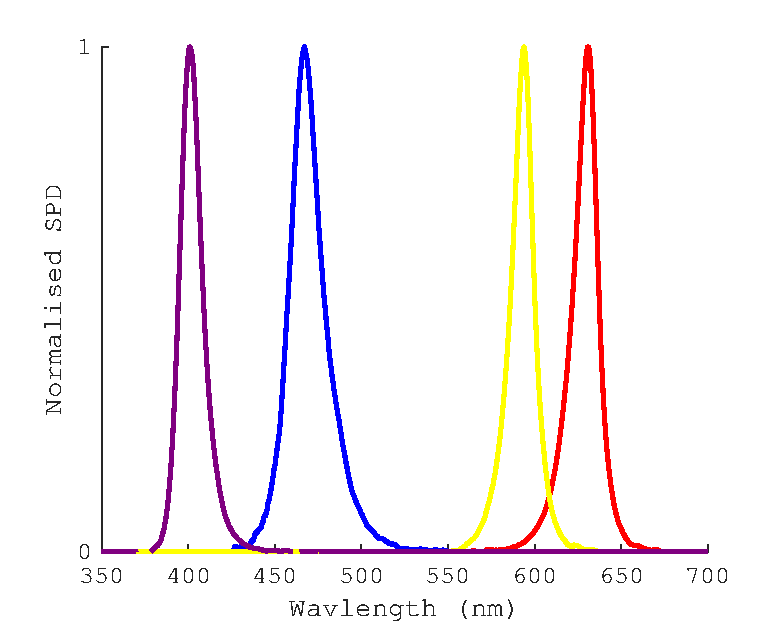
\includegraphics[max width=\textwidth,center]{figs/SmallSphere/LED_SPDs.pdf}
\caption{The normalised \glspl{SPD} of the Small Sphere \glspl{LED}, with lines connecting the pairs which were activated simultaneously.}
\label{fig:LED_SPDs}
\end{figure}

The arduino script set the \glspl{LED}, via pulse width modulation, to the output levels decided in the perceptual nulling segment of the experiment. The two modes had either the combination of UV and amber, or blue and red, allowing for the chromaticities falling upon the lines shown in Figure \ref{fig:LED_SPDs}. The combinations UV and blue, or amber and red, were never used.

\begin{figure}[htbp]
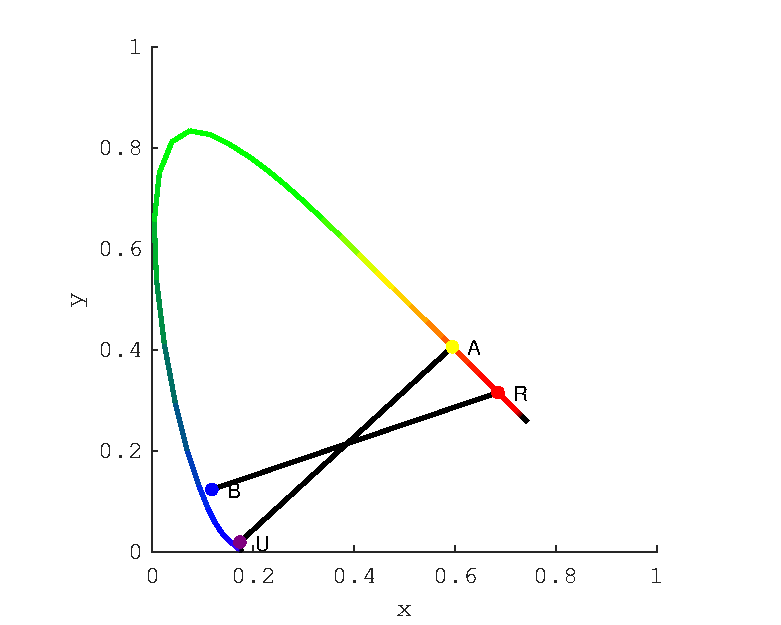
\includegraphics[max width=\textwidth,center]{figs/SmallSphere/LED_cross.pdf}
\caption{The chromaticities of the Small Sphere \glspl{LED} in CIE 1931 space. Thus from each pair, illumination with chromaticity values extending along each line was generatable. Even if there were differences in the spectral sensitivities of the observers (compared to the CIE 1931 observer), with these narrow-band primaries there should theoretically always be a point at which the two lines cross.}
\label{fig:LED_cross}
\end{figure}

This breadboard was mounted stably atop the sphere with a perspex diffusion sheet between it and the opening into the sphere. Black card was used to mask stray light, mainly to address the specific concern that light may fall onto the LCD display.

%LM: photo of the construction of the lighting rig (close up)

Throughout the experiments the illumination inside the sphere was measured with an Ocean Optics USB 2000+ through a optical fiber probe mounted to the base of the sphere and directed at a point on the roof of the sphere, opposite the observer. It was expected that the output of the \glspl{LED} may change slightly over time. %fig x?

\subsubsection{Light safety}
Since illumination of wavelengths shorter than 400nm would be present, it was deemed appropriate to take extra precautions to ensure the safety of participants. 
The implementation of the `BS EN ISO 15004-2:2007 Ophthalmic instruments - Fundamental requirements and test methods - Part 2: Light hazard protection' \citep{iso/tc_172/sc_7_ophthalmic_optics_and_instruments_bs_2007} provided in the Silent Substitution toolbox\footnote{\url{https://github.com/spitschan/SilentSubstitutionToolbox}} created by \citet{spitschan_selective_2015} was used to evaluate the safety of the experimental set-up, and under the default assumptions for pupil size, and with the maximum output from the LEDs, the stimulus was found to be considerably below the limits for type 1 continuous wave instruments. See Appendix \ref{app:ethics3} for further details.

% safety
% The controllers 
% The code
% Characterisation / ongoing measurement

\subsection{Observer task}

\subsubsection{Perceptual Nulling}

The basic logic of this experiment is as follows: under the null hypothesis two adapting fields of identical appearance should cause an observer to be adapted in exactly the same way. In order to design two adapting field illuminants which appear identical (perceptual metamers) we can either make predictions based upon standard observers (with parameters set to match our real observers regards age and pupil dilation etc.) or we can employ a process whereby individual observers make minor alterations to two conditions, that are designed such that they could be metamers, until they appear identical. We have opted to use colorimetry as a starting point to choose primaries (Figure \ref{fig:LED_cross}), and then allow observers to fine-tune this matching.

We run the risk of falling into circularity here: we ask observers to set two fields such that they appear identical, and then (in a roundabout way) we ask them whether there is any visual difference between them. If melanopsin does have a direct impact upon visual perception we are at risk of accounting for this at this stage. In an attempt to avoid this problem, we perform the perceptual nulling under conditions which we predict should not allow for \gls{ipRGC} involvement, or should minimise such. It seems to be the case that \glspl{ipRGC} do not react strongly over very short timescales ($<$0.5hz \citep{spitschan_human_2017-1}), with cones being much more active in this temporal window, so we chose to alternate rapidly between the two conditions and ask observers to make alterations until there is a minimal visible flicker.

Observers were instructed to fixate upon a small fixation point displayed at the centre of the otherwise dark display. They placed their hands upon three dials which could be independently varied to change the peripheral adapting illumination inside the sphere.

Two modes were presented to observers, one where the two conditions were alternated at 30hz for 1 second, followed by a 10 second break, and one where the conditions were alternated at 4hz for 500ms, followed by a 1 second break. 

During the first condition the observer was requested only to alter the setting of the first dial, which would change the overall level of the red/blue combination (whilst the uv/amber combination remained at the same level). This was referred to as brightness matching.

During the second condition the observer was requested only to alter the settings of the second and third dials. The second dial would alter the relative contributions of red/blue to the first condition. The third dial would alter the relative contributions of uv/amber to the second condition. These options can be thought of as traversing the straight lines in Figure \ref{fig:LED_cross}. This was referred to as colour matching.

%LM: photo of observer looking into sphere

The observer was allowed to switch back and forth between these two modes until they were happy with the match. Once an observer had indicated a match, the LED drive values were recorded and these were used for the observer in future sessions.

Observers found this task rather arduous, predominantly due to the inherent difficulty in making colour matches in the periphery. An additional difficulty was that since eye movements were not strictly controlled, if an observer were briefly to look away from the fixation they would be able to see the adapting field with their foveal vision. This was problematic since in most cases the peripheral matches induced strong contrast for foveal perception. Though it was unintentional, this seems to be a particularly effective way of generating the perception of a Maxwell spot \citep{isobe_functional_1955}. Further to this, the authors' experience was that the visible periphery could be further divided, by eccentricity, into two or possibly three areas where a match in one area would not provide a match in both areas.

Despite these difficulties, observers generally found settings which for them resulted in a metameric match (where they could no longer perceive flicker, or perceived minimal flicker). One observer who initially agreed to be part of the study withdrew at this stage, partly due to a difficulty completing this task, but mainly due to a claustrophobic reaction. Another potential observer withdrew at this stage, since he was unable to make a match using this set of primaries, which we tentatively attribute to incipient cataracts.

This method has since been further developed by \citet{allen_form_2019} who used a 2AFC task instead of a method of manual adjustment to pinpoint areas of perceptual metamerism.

% Observers were...
% Initial metamer setting
\subsubsection{Achromatic selections}

3 observers took part in the main experiment (the author (DG), HC, and LW). 

The task was identical to that performed in the Large Sphere experiment; using two sliders (controlling the yellow/blue component and the red/green component) to set the foveal stimulus to appear achromatic. As previously noted, instead of 10 runs of L* 85 descending in 5* increments to L* 10, there were 30 runs of a pseudo-randomly permuted (each run) set of stimuli specified such that there was one at every 10 L* interval between 30 L* and 70 L*. The range was reduced so as to minimise the impact of gamut-boundary issues. The L* interval was increased to allow for a greater number of repetitions of specific values within a similar time frame. The order was pseudo-randomly permuted to avoid any trend based effects.

Two observers (HC and LW) performed 4 complete runs each, 2 under each condition. The author completed 2 runs, one under each condition. Each observer only completed one run per day. There was a gap of roughly three months between the initial runs of HC and LW and the repeat runs.

\subsubsection{Data Analysis}

Following calibration, for each observer under each condition, the means and standard deviation were computed for each dimension of CIELAB. The inter-condition mean vectors were calculated.

The data were submitted to a two-sample two-dimensional Kolmogorov-Smirnov test\footnote{Using the function available from \url{https://uk.mathworks.com/matlabcentral/fileexchange/38617-kstest_2s_2d-x1-x2-alpha}.} to compare the two distinct conditions for each observer (including data for repeats where performed). 

To provide a baseline-check, the same test was applied to the repeat data for two observers, with the assumption that this would not return a significant difference.

These results were considered alongside measurements of LEDs taken during the experiments.

\section{Results}

\subsection{Primary Data}

A summary of results, where each run is represented by a standard deviation ellipse, is shown in Figure \ref{fig:SSsummary}. Break downs for each observer, showing each achromatic setting are shown in Figures \ref{fig:SS_DG} - \ref{fig:SS_LW}.

\begin{figure}[htbp]
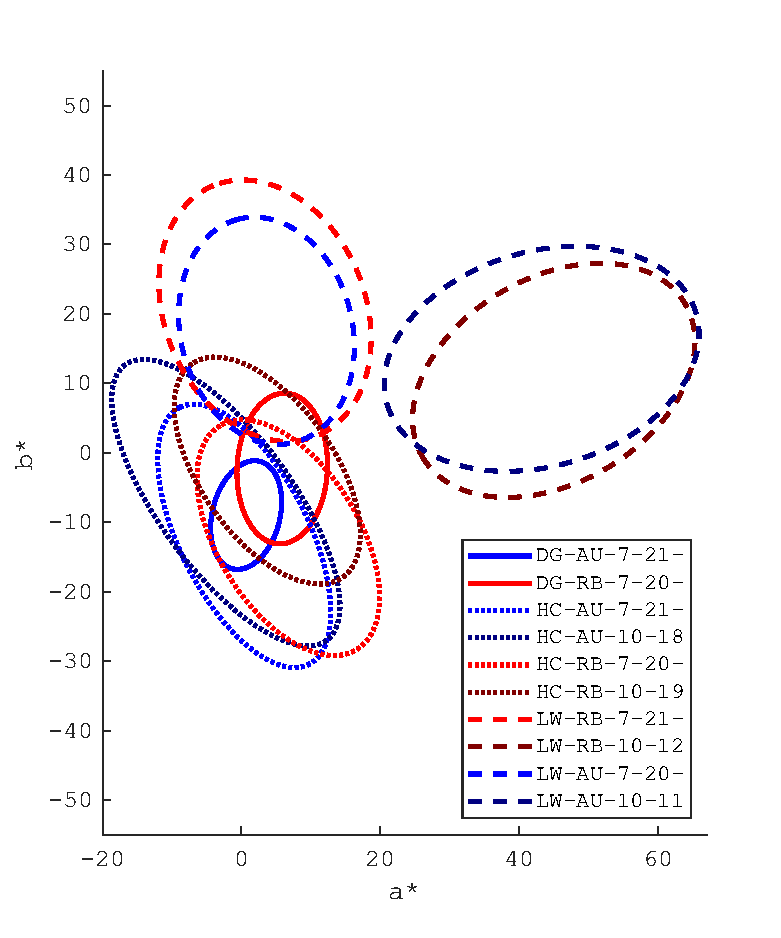
\includegraphics[max width=\textwidth,center]{figs/SmallSphere/SSsummary.pdf}
\caption{}
\label{fig:SSsummary}
\end{figure}

\begin{figure}[htbp]
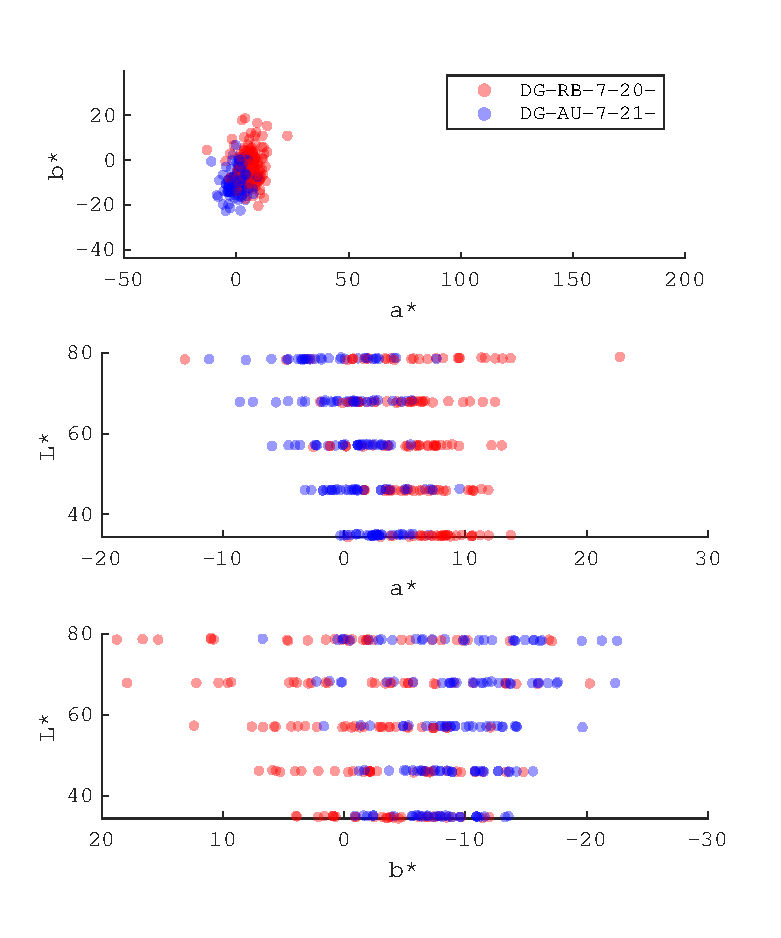
\includegraphics[max width=\textwidth,center]{figs/SmallSphere/DG.pdf}
\caption{}
\label{fig:SS_DG}
\end{figure}

\begin{figure}[htbp]
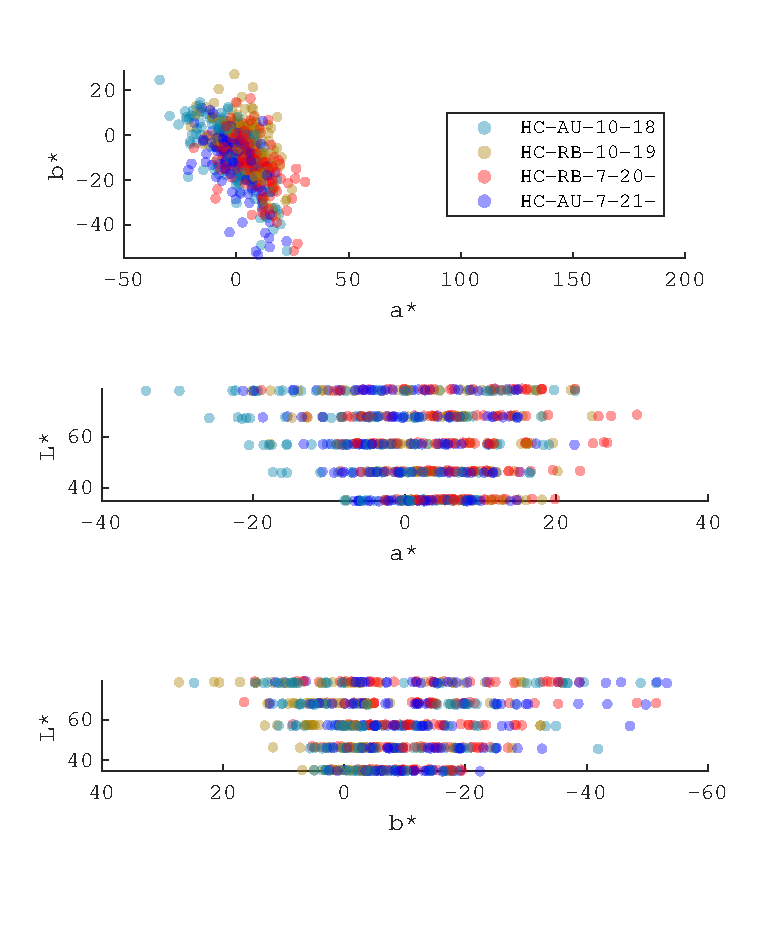
\includegraphics[max width=\textwidth,center]{figs/SmallSphere/HC.pdf}
\caption{}
\label{fig:SS_HC}
\end{figure}

\begin{figure}[htbp]
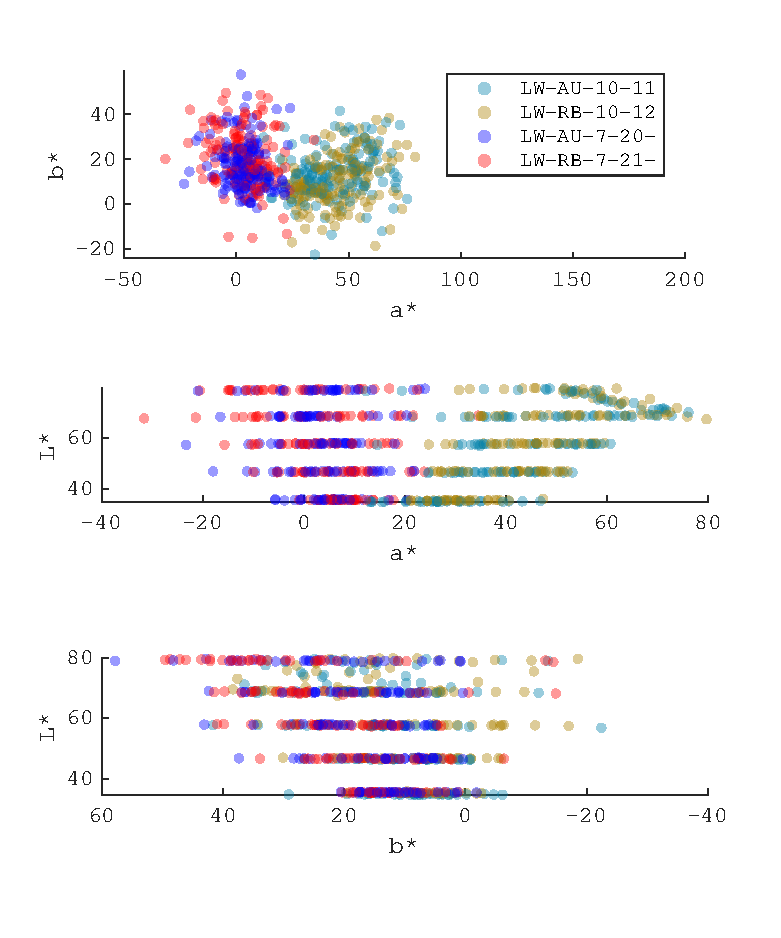
\includegraphics[max width=\textwidth,center]{figs/SmallSphere/LW.pdf}
\caption{}
\label{fig:SS_LW}
\end{figure}

\subsection{Secondary Data}

Data describing the characterisations of hardware follow. Figure \ref{fig:SSLEDs} shows the chromaticities of the adapting surrounds as recording during each session. Figure \ref{fig:SSgamut} shows the recorded gamut and white points of the display measured before or after each session. Figure \ref{fig:SScal2} shows representative results from one of the secondary characterisation sessions.

\begin{figure}[htbp]
%\includegraphics[max width=\textwidth,center]{figs/SmallSphere/SSLEDs.pdf}
\caption{}
\label{fig:SS_LW}
\end{figure}

\begin{figure}[htbp]
%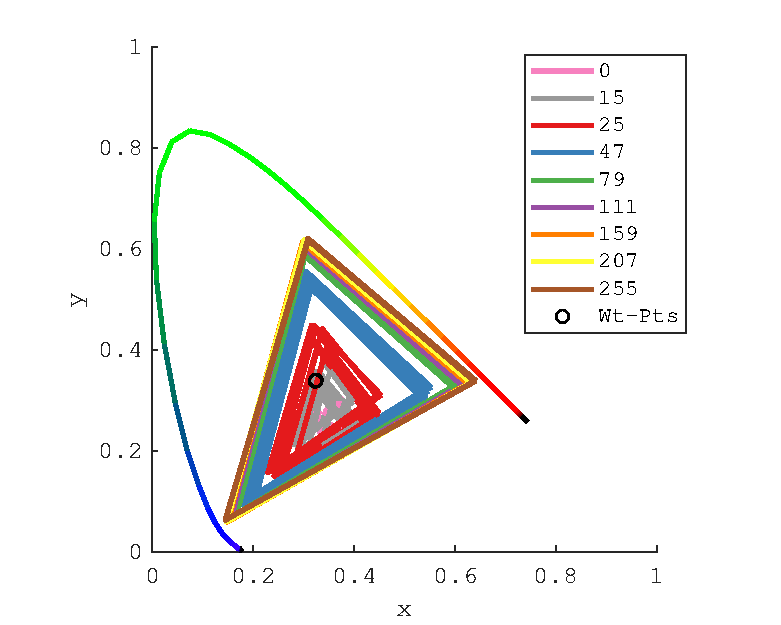
\includegraphics[max width=\textwidth,center]{figs/SmallSphere/SSgamut.pdf}
\caption{}
\label{fig:SS_LW}
\end{figure}

\begin{figure}[htbp]
%\includegraphics[max width=\textwidth,center]{figs/SmallSphere/SScal2.pdf}
\caption{}
\label{fig:SS_LW}
\end{figure}

\section{Discussion}
% Assumptions

%Rod activation
%Calculate melanopic contrast for actual conditions
%Line indicates match
